\section{Experimental results and discussions}
\label{sec:experimental_results}
In order to show the accuracy of the proposed model of EM reliability for multi-branch interconnect three with line structure shown in Fig. \ref{fig:interconnect_tree}, the analytical solution \eqref{eq:general_solution} of stress evolution equations is calculated with the MATLAB enviroment, and we also compare the results from \eqref{eq:general_solution} with those obtained by the finite element tool COMSOL \cite{COMSOL}. In our experiments, we test two cases of interconnect tree structure by changing $n$ in \eqref{eq:general_solution} which is the number of wire segments in the interconnect tree. In the simulations to be described below, the following parameter values will be used: $Z^*=10$, $\rho=3\times10^{-8} \Omega/m$, $\Omega=8.78\times10^{-30}m^3$, $B=5.5\times10^{10} Pa$, $D_0=5.5\times10^{-5} m^2/s$, $E_a=1.1eV$, $e=1.6\times10^{-19}C$, $k=1.38\times10^{-23}J/K$ , and $T=350K$.

\subsection{Four-terminal interconnect wire ($n=3$)}
\begin{figure}[!h]
\centering
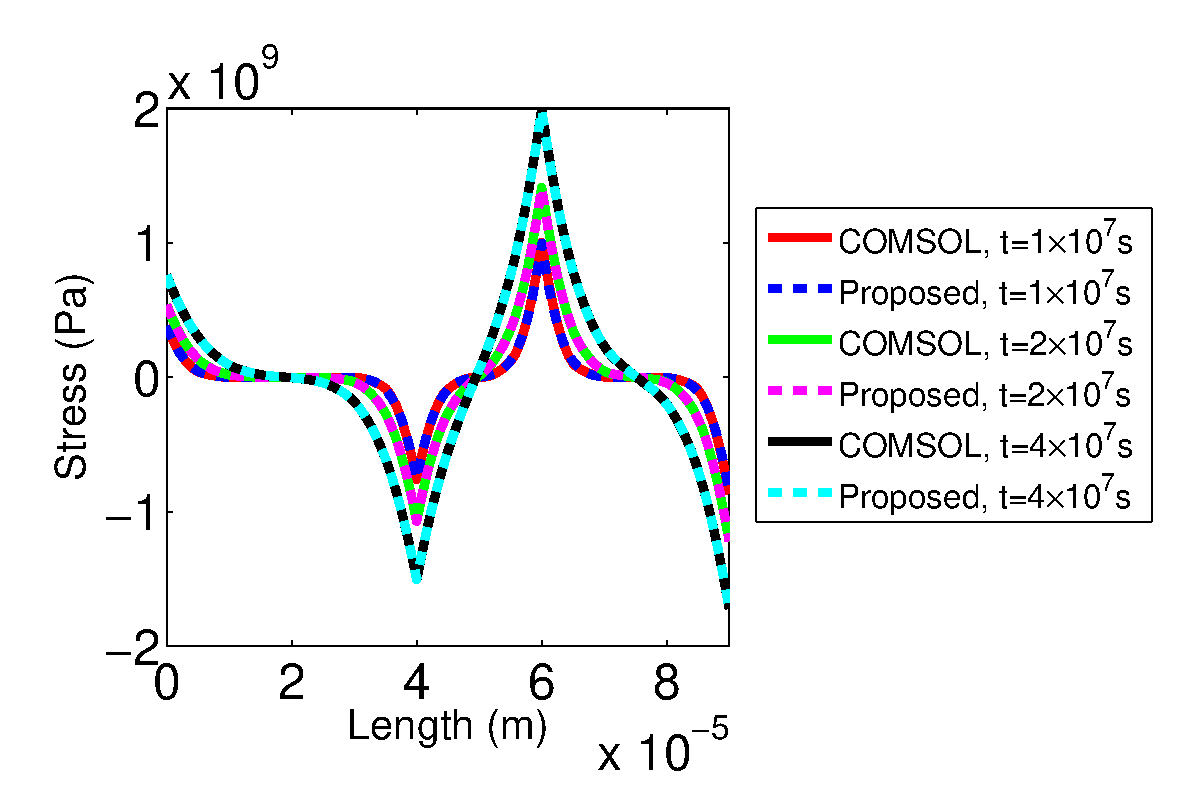
\includegraphics[width=0.9\columnwidth]{S3StressMatComCompareT0.eps}
\caption{EM-induced stress evolution along the four-terminal interconnect wire ($n=3$).}
\label{fig:S3StressMatComCompare}
\end{figure}
We first analyze the four-terminal interconnect tree with three wire segments with the current flow directions as shown in Fig. \ref{fig:interconnect_tree}. For this type of interconnect wire, the integer $n$ in the stress evolution equation \eqref{eq:general_interconnect_tree} is set to be 3. For our simulation, a constant current density of $j_1=2.2\times 10^{10}A/m^2$ is applied in the left segment, while a current density with varying direction and magnitude, $j_2=-6.6\times 10^{10}A/m^2$ is used to stress the middle wire segment. The current density of the right wire segment is set to be $j_3=5\times 10^{10}A/m^2$. The lengths for this four-terminal interconnect wire are set to be $l_0=0\times 10^{-5}m$, $l_1=4\times 10^{-5}m$, $l_2=6\times 10^{-5}m$, and $l_3=9\times 10^{-5}m$, respectively. Fig. \ref{fig:S3StressMatComCompare} shows the EM stress development calculated by employing the one-term approximation form of the exact series solution \eqref{eq:general_solution} for the three-segment interconnect wire, in comparison with the finite element analysis results obtained from COMSOL. It can be seen from Fig. \ref{fig:S3StressMatComCompare} that the analytical solution obtained with the proposed method fits well to the results of the numerical simulation at every time instance.

\begin{figure}[!h]
\centering
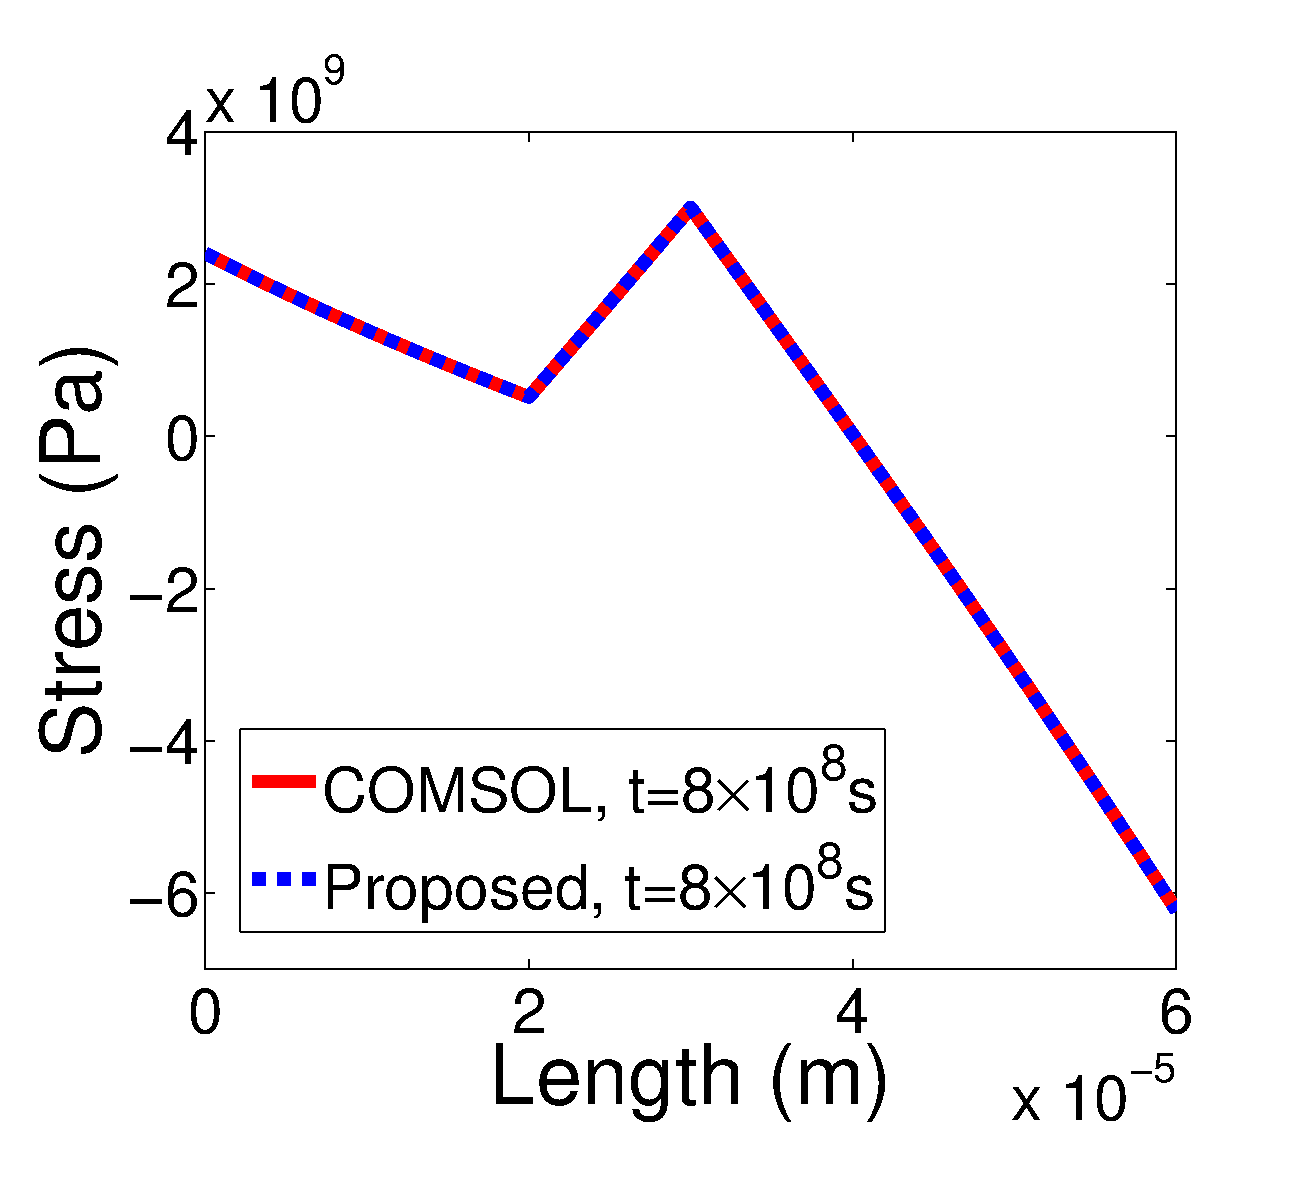
\includegraphics[width=0.7\columnwidth]{S3StableT0.eps}
\caption{Steady-state stress distributions along the four-terminal interconnect wire ($n=3$).}
\label{fig:S3StableT0}
\end{figure}

\begin{figure}[!h]
\centering
\subfigure[]{
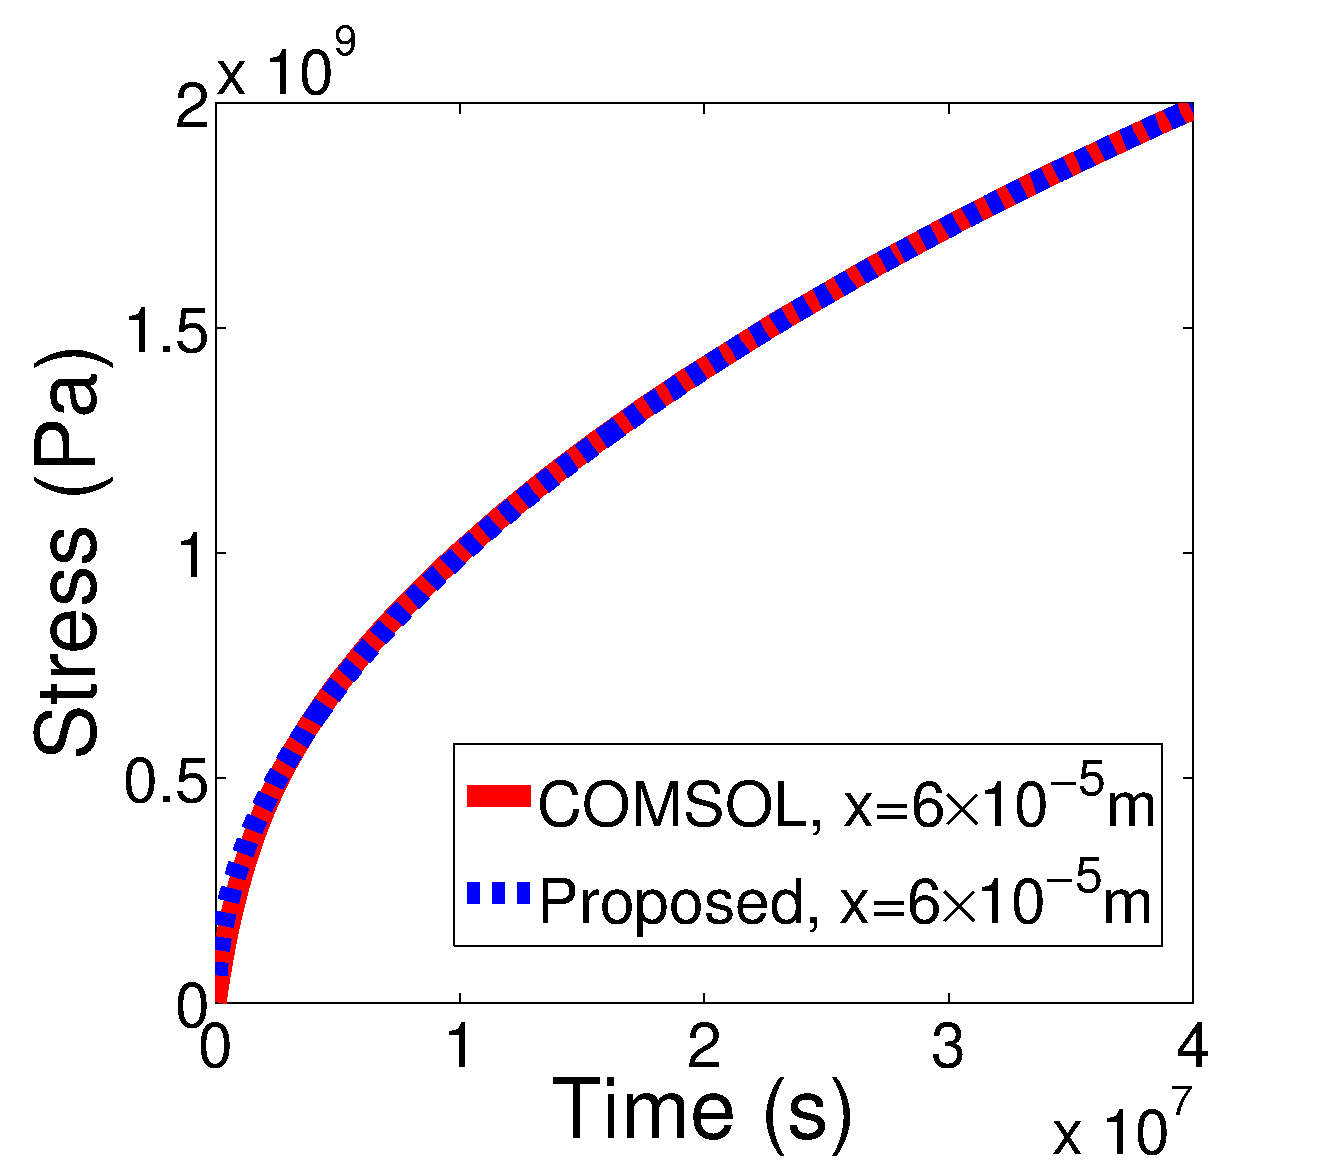
\includegraphics[width=0.45\columnwidth]{S3LengthCompare6T0.eps}
\label{fig:S3point1}}
\subfigure[]{
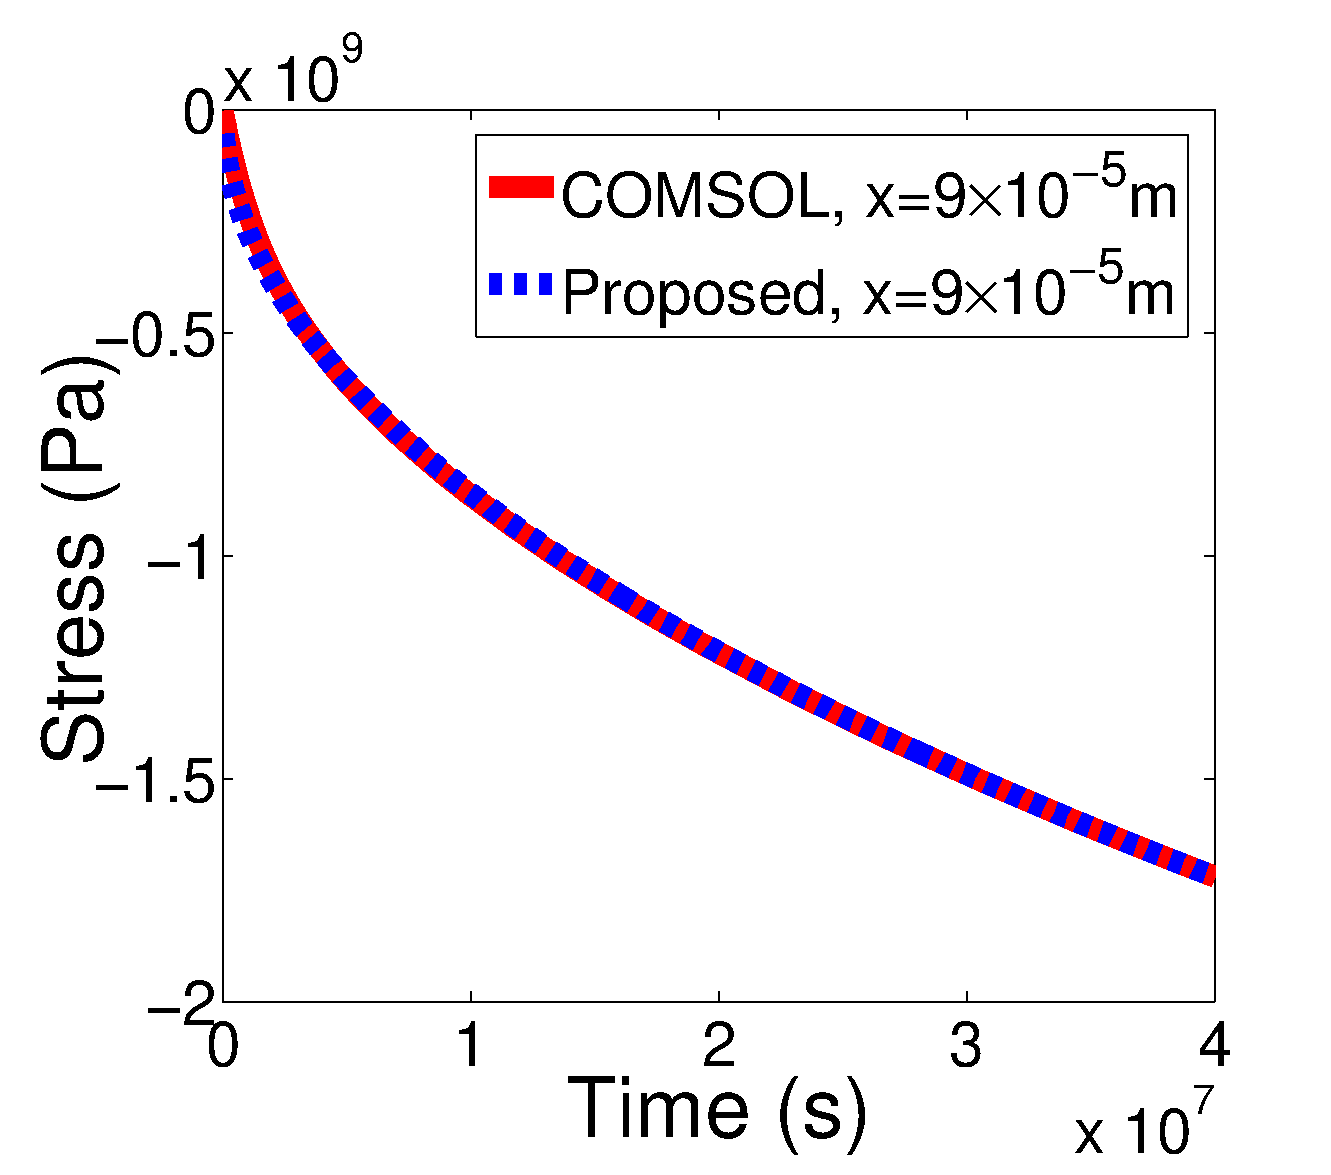
\includegraphics[width=0.45\columnwidth]{S3LengthCompare9T0.eps}
\label{fig:S3point2}}
\caption{EM-induced stress development over time for the four terminal interconnect wire: (a) the tensile stress at the position $x=6\times 10^{-5}m$; (b) the compressive stress at the position $x=9\times 10^{-5}m$.}
\label{fig:S3Results2}
\end{figure}

Localized tensile and compressive stresses are generated from the EM-induced material depletion and accumulation at the locations of atom flux divergence. The resulting stress gradient leads to a backflow flux of atoms to oppose the EM flux. For the void nucleation phase, EM-induced voids will not form if the balance between the backflow and EM fluxes can be achieved before the tensile stress value along the metal wire reaches the critical stress boundary. In this situation, the wire interconnect structure is virtually immortal. The wire will be immortal if the maximum steady-state stress is less than the critical stress $\sigma_{crit}$. It is observed from Fig. \ref{fig:S3StableT0} that the steady-state stress distributions from the proposed analytical model matches well with the COMSOL simulation results.

It should be noted that the current direction in the middle segment is opposite to the direction of the currents in the left and right segments. As a result, both the tensile and compressive stresses can be generated along this three-segment interconnect wire. Fig. \ref{fig:S3point1} and Fig. \ref{fig:S3point2} show the developments of the tensile stress at the position $x=6\times 10^{-5}m$ and the compressive stress at the position $x=9\times 10^{-5}m$, respectively. It can be seen from Fig. \ref{fig:S3Results2} that both the tensile and compressive stressed calculated by the proposed analytical model matches well the COMSOL simulation results.


\subsection{Six-terminal interconnect wire ($n=5$)}
\begin{figure}[!h]
\centering
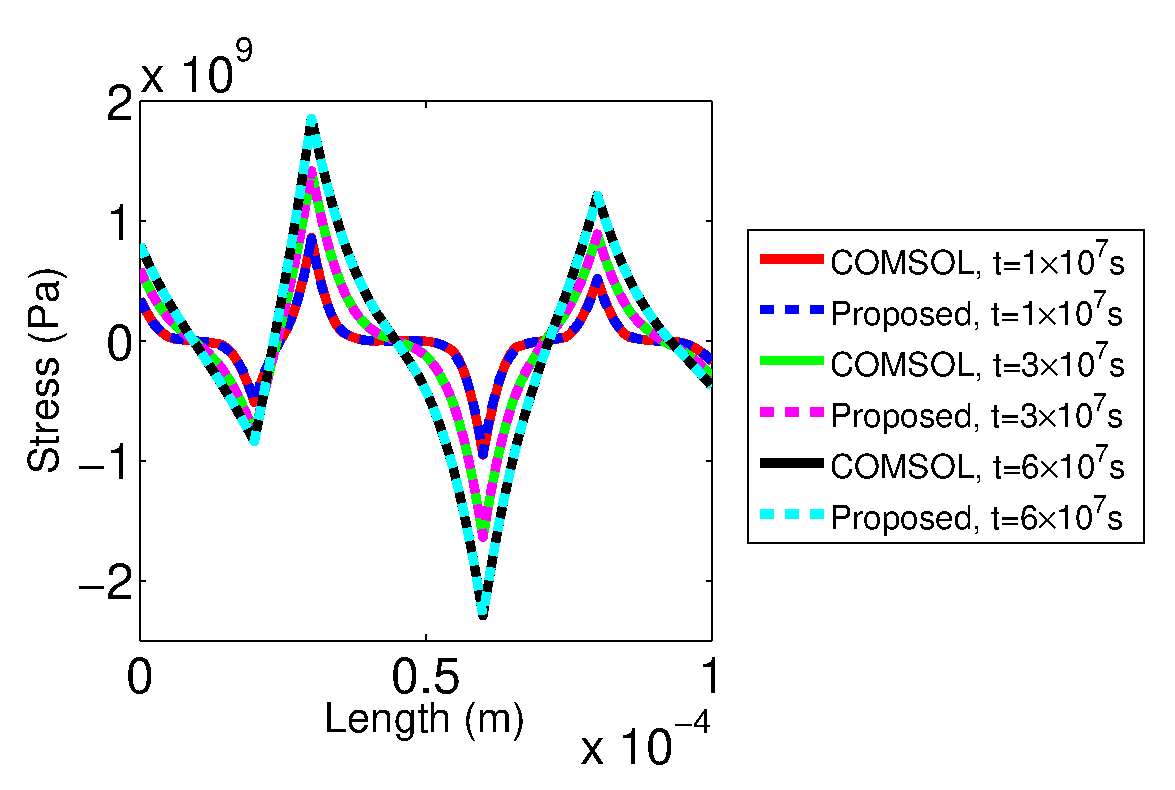
\includegraphics[width=0.9\columnwidth]{S5StressMatComCompareT0.eps}
\caption{EM-induced stress development along the six-terminal interconnect wire ($n=5$).}
\label{fig:S5StressMatComCompare}
\end{figure}
Now we calculate the EM-induced stress evolution by the proposed analytical model for the six-terminal interconnect wire. For this type of interconnect wire, the integer $n$ in the closed-form expression \eqref{eq:general_solution} equals to 5. For the simulation of stress evolution during the void nucleation phase, the current densities in each segment are set to be $j_1=2\times 10^{10}A/m^2$, $j_2=-4\times 10^{10}A/m^2$, $j_3=6\times 10^{10}A/m^2$, $j_4=-5\times 10^{10}A/m^2$, and $j_5=1\times 10^{10}A/m^2$, respectively. The lengths $l_i(i=0,1,\cdots,5)$ in \eqref{eq:general_solution} for this five-segment wire are chosen as $l_0=0\times 10^{-5}m$, $l_1=2\times 10^{-5}m$, $l_2=3\times 10^{-5}m$, $l_3=6\times 10^{-5}m$, $l_4=8\times 10^{-5}m$, and $l_5=10\times 10^{-5}m$, respectively. We use the one-term approximation of the exact series solution \eqref{eq:general_solution} to calculate the EM-induced stress development along this five-segment wire. Fig. \ref{fig:S5StressMatComCompare} shows the time evolution of the stress during the void nucleation phase. It can be seen from Fig. \ref{fig:S5StressMatComCompare} that the obtained results are in good agreement with the finite element simulation results.

As mentioned above, if the critical stress $\sigma_{crit}$ during the void nucleation phase is greater than the maximum steady-state tensile stress value along the five-segment interconnect wire, it is immortal, i.e., no voids will form in the wire and it will never fail. Fig. \ref{fig:S5StableT0} shows the steady-state stress distributions along the wire, from which we can see that the analytical solution can fit well with the COMSOL simulation results. It should be noted that the first, third, and fifth segments in the line wire have the same current direction that is opposite to the direction of the currents in the second and fourth segments. As a result, both the tensile and compressive stresses can be generated in this interconnect wire. Fig. \ref{fig:S5point1} and Fig. \ref{fig:S5point2} show the compressive stress development over time at the position $x=6\times 10^{-5}m$ and the tensile stress development at $x=8\times 10^{-5}m$, respectively. Again, the obtained results from the one-term approximation of the exact series solution match well with the numerical simulation results calculated by COMSOL.

\begin{figure}[!h]
\centering
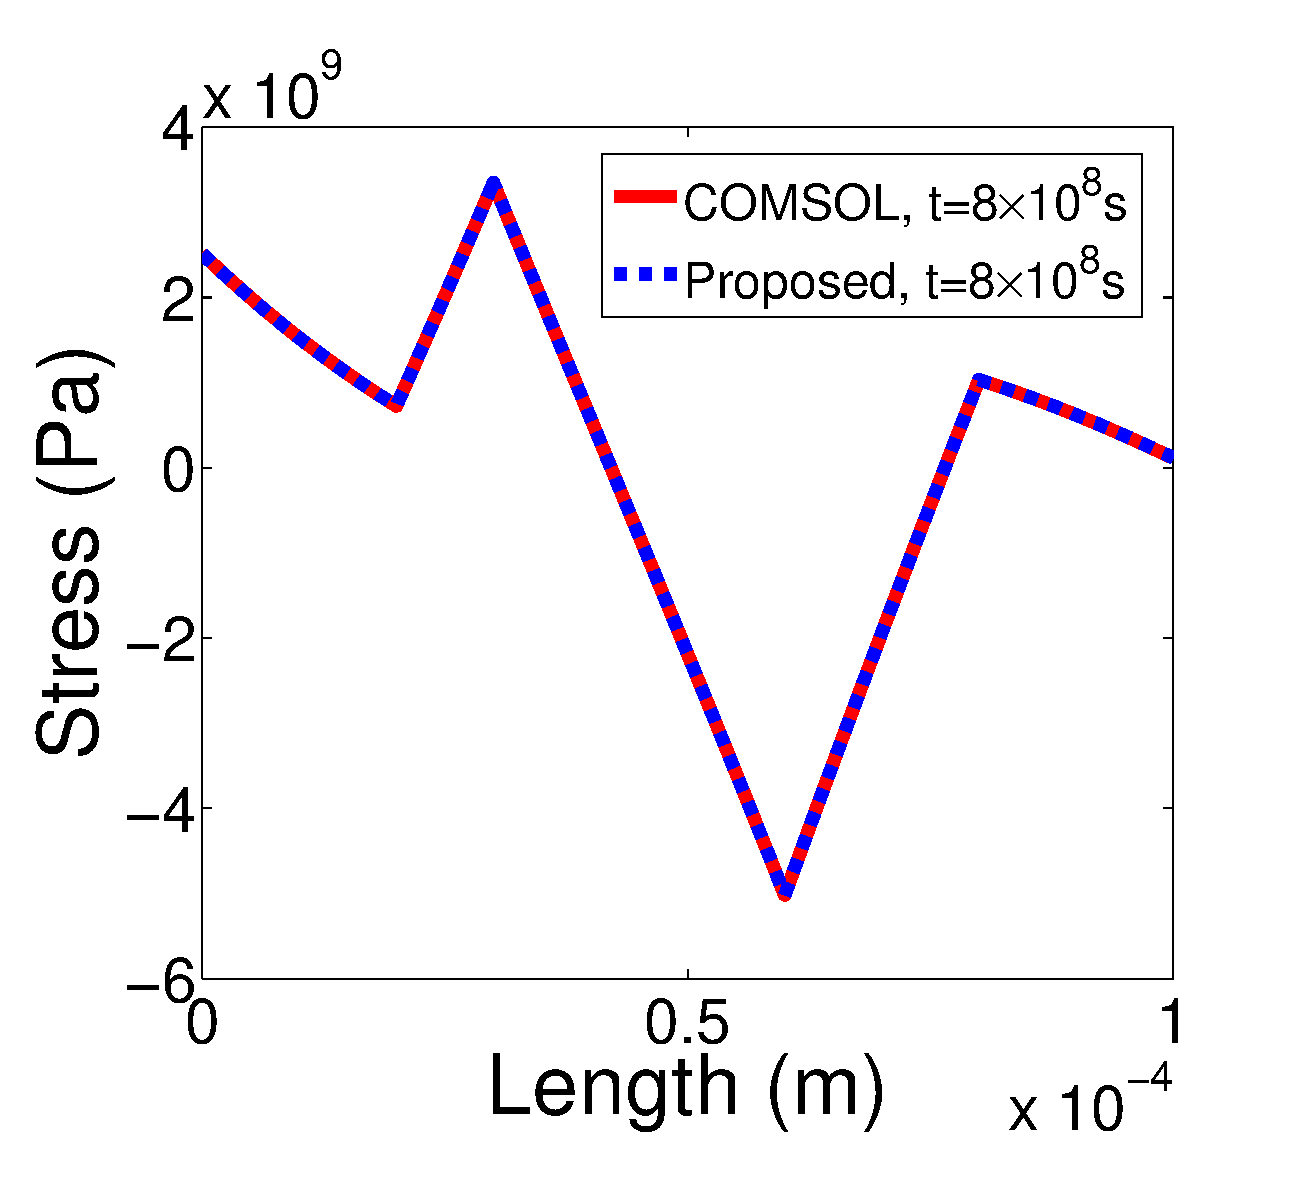
\includegraphics[width=0.7\columnwidth]{S5StableT0.eps}
\caption{Steady-state stress distributions along the six-terminal interconnect wire ($n=5$).}
\label{fig:S5StableT0}
\end{figure}

\begin{figure}[!h]
\centering
\subfigure[]{
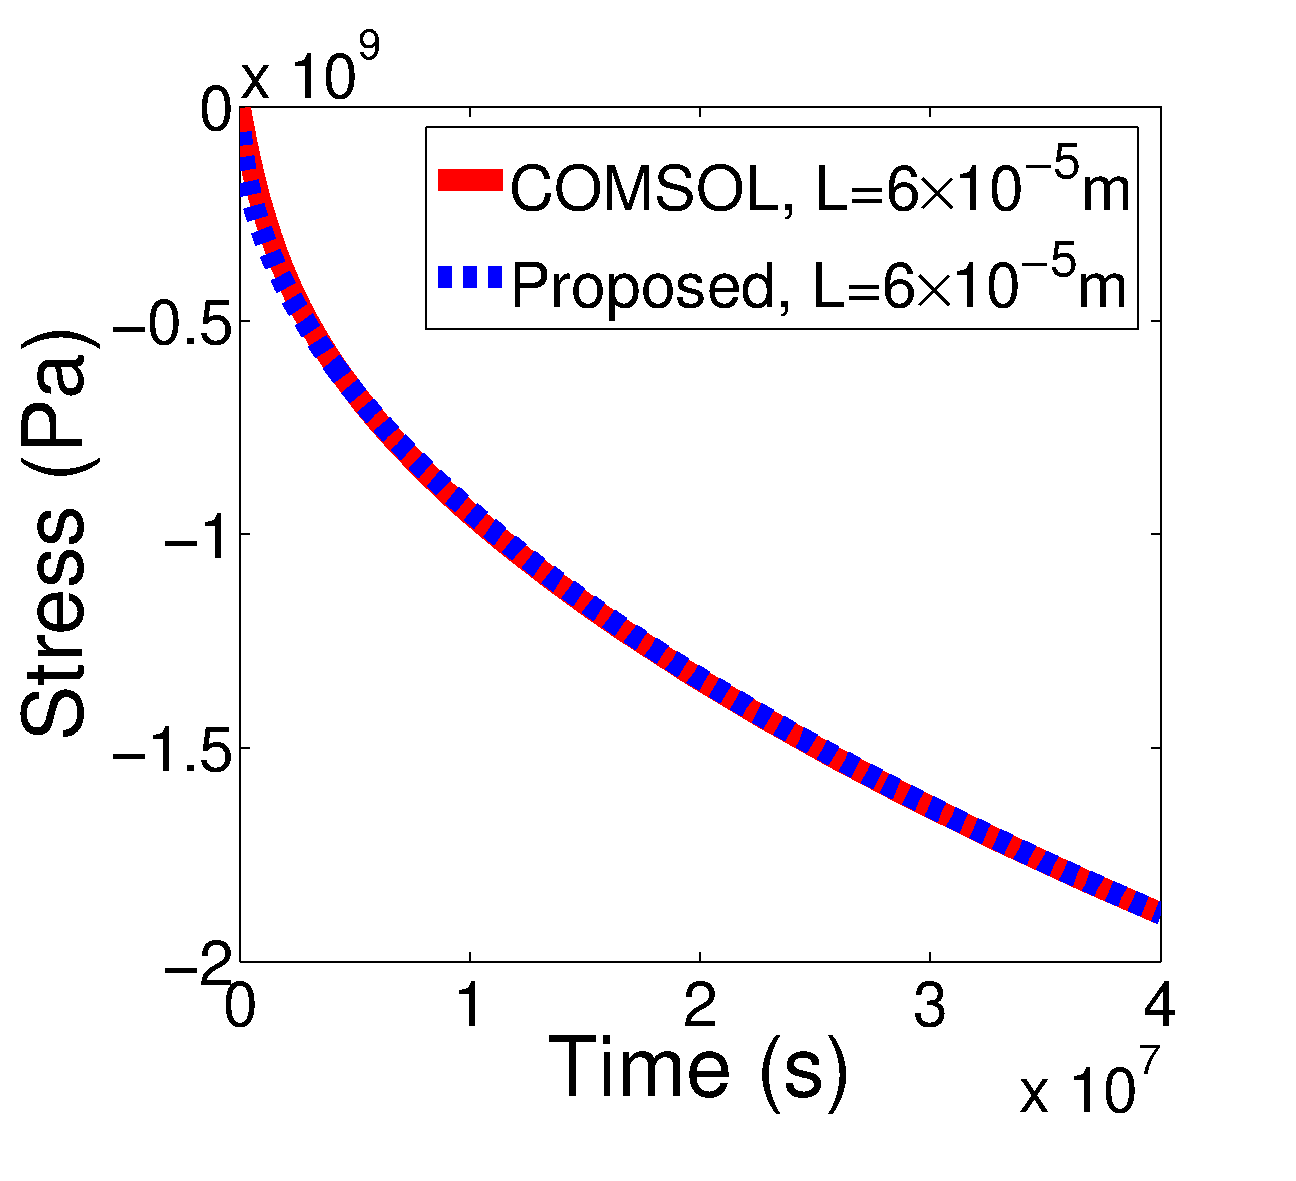
\includegraphics[width=0.45\columnwidth]{S5LengthCompare6T0.eps}
\label{fig:S5point1}}
\subfigure[]{
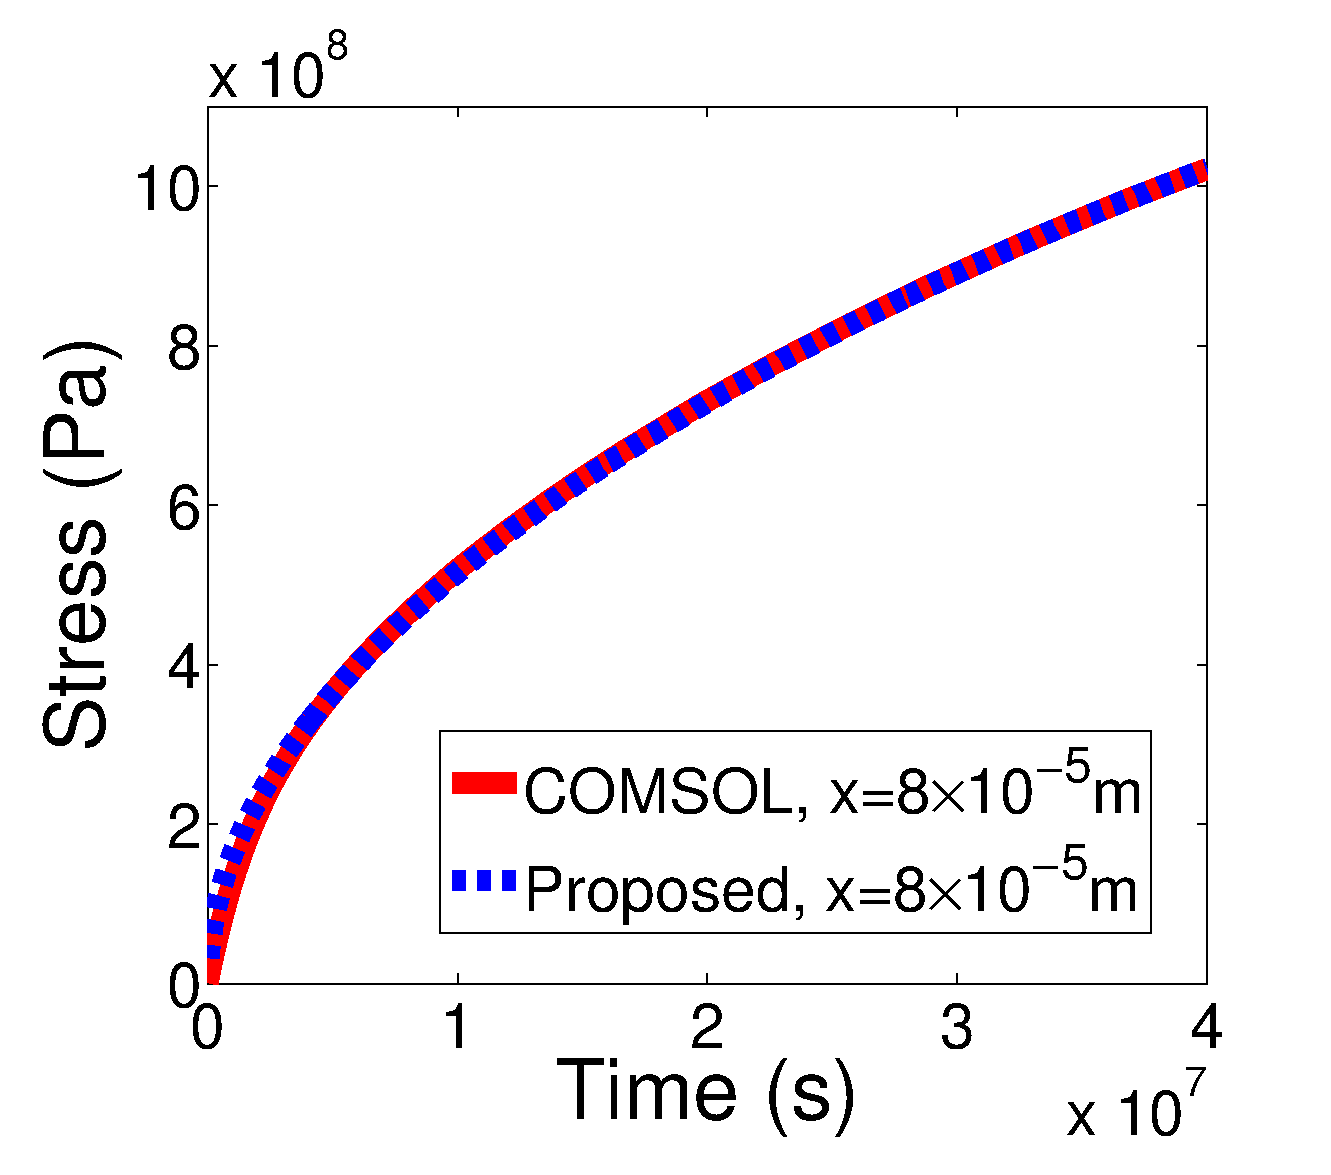
\includegraphics[width=0.45\columnwidth]{S5LengthCompare8T0.eps}
\label{fig:S5point2}}
\caption{EM-induced stress development over time for the six-terminal interconnect wire: (a) the compressive stress at the position $x=6\times 10^{-5}m$; (b) the tensile stress at the position $x=8\times 10^{-5}m$.}
\label{fig:S5Results2}
\end{figure}


\subsection{Accuracy study for the analytic model}
We now study the accuracy of the proposed analytic model using the one-term approximation of the exact series solution against the COMSOL simulation results.
Due to limited space, only the results for the three-segment wire case are shown in the paper. The relative errors are plotted in Fig. \ref{fig:TimeError1e8} against the COMSOL simulation results for the case using the one-term approximation, i.e., the integer $m$ in the series solution \eqref{eq:general_solution} is set to be zero. As we can see from Fig. \ref{fig:TimeError1e8}, the resulting relative errors between the one-term approximation and the COMSOL simulation results are around 2\%. In the experiments we noted that the accuracy cannot be improved significantly by adding more terms, which means that the one-term approximation is enough to calculate the EM-induced stress during the void nucleation phase for this three-segment interconnect tree.
\begin{figure}[!h]
\centering
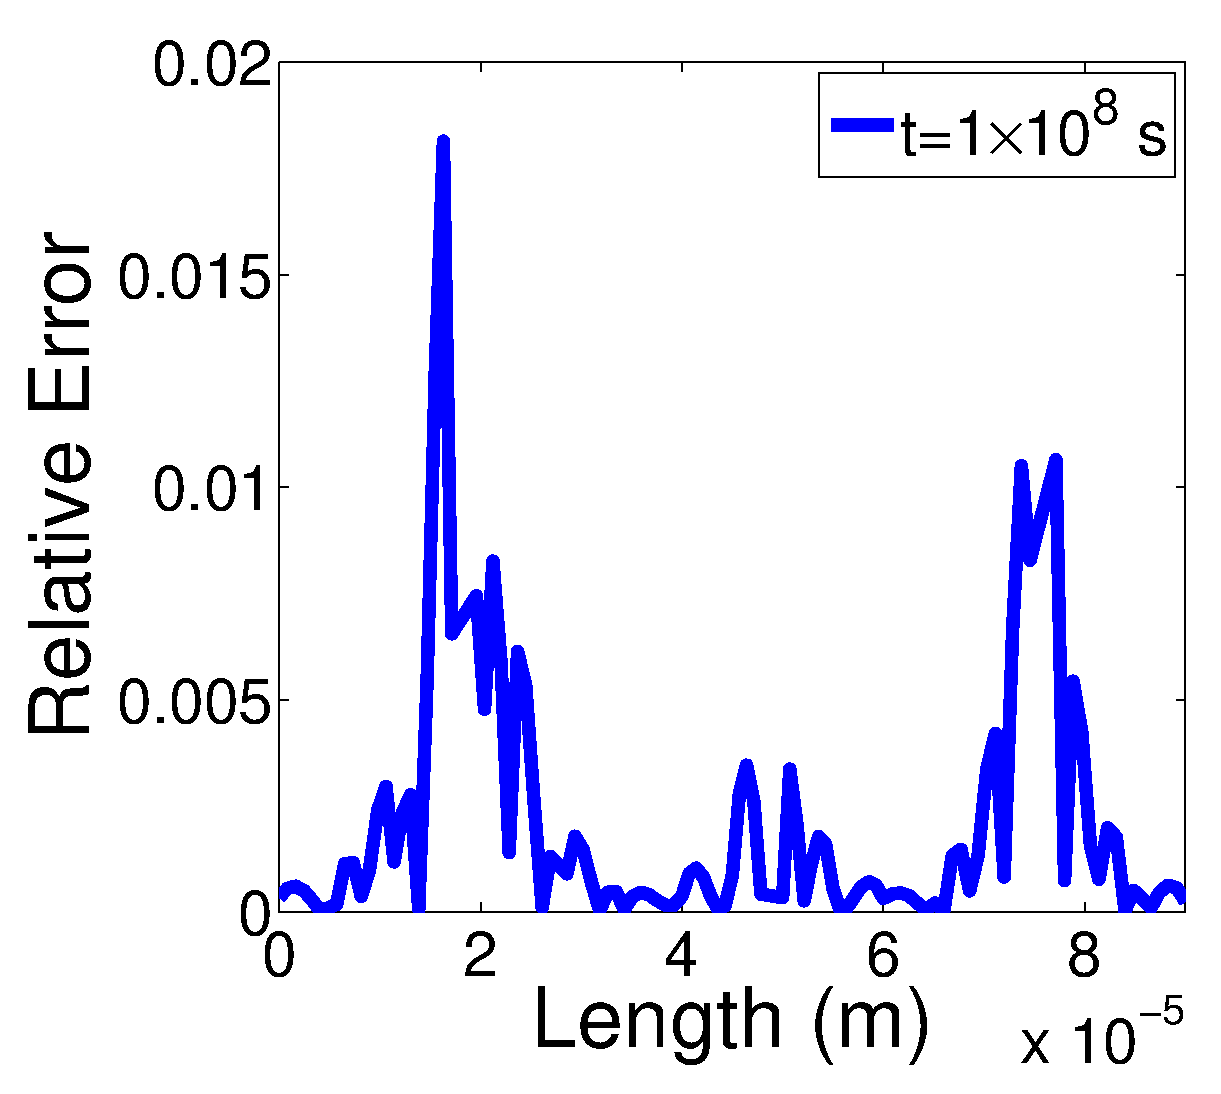
\includegraphics[width=0.7\columnwidth]{TimeError1e8.eps}
\caption{Relative errors between the proposed analytical model and the
COMSOL model for the three-segment interconnect wire.}
\label{fig:TimeError1e8}
\end{figure}

